\documentclass{entcs} \usepackage{entcsmacro}
\usepackage{graphicx}

% The following is enclosed to allow easy detection of differences in
% ascii coding.
% Upper-case    A B C D E F G H I J K L M N O P Q R S T U V W X Y Z
% Lower-case    a b c d e f g h i j k l m n o p q r s t u v w x y z
% Digits        0 1 2 3 4 5 6 7 8 9
% Exclamation   !           Double quote "          Hash (number) #
% Dollar        $           Percent      %          Ampersand     &
% Acute accent  '           Left paren   (          Right paren   )
% Asterisk      *           Plus         +          Comma         ,
% Minus         -           Point        .          Solidus       /
% Colon         :           Semicolon    ;          Less than     <
% Equals        =3D           Greater than >          Question mark ?
% At            @           Left bracket [          Backslash     \
% Right bracket ]           Circumflex   ^          Underscore    _
% Grave accent  `           Left brace   {          Vertical bar  |
% Right brace   }           Tilde        ~

% A couple of exemplary definitions:

\newcommand{\Nat}{{\mathbb N}}
\newcommand{\Real}{{\mathbb R}}
\def\lastname{Luukkainen}
\begin{document}
\begin{frontmatter}
  \title{Verifying a UMTS protocol using Spin and EASN}
  \author{Matti Luukkainen\thanksref{mattiEmail}}
  \address{University of Helsinki, Department of Computer Science
	P.O.Box 26, 00014 University of Helsinki, Finland}
  \author{Vivek K. Shanbhag\thanksref{vivekEmail}}
  \address{Sun Microsystems, Divyasree Chambers, Bangalore 560025}
  \author{K. Gopinath\thanksref{gopiEmail}}
  \address{CSA Dept, Indian Institute of Science, Bangalore 560012}
  \thanks[mattiEmail]{Email: \href{mailto:mluukkai@cs.helsinki.fi}
    {\texttt{\normalshape mluukkai@cs.helsinki.fi}}}
  \thanks[vivekEmail]{Email: \href{mailto:vivek.shanbhag@sun.com}
    {\texttt{\normalshape vivek.shanbhag@sun.com}}}
  \thanks[gopiEmail]{Email: \href{mailto:gopi@csa.iisc.ernet.in}
    {\texttt{\normalshape gopi@csa.iisc.ernet.in}}}

\begin{abstract} 
Next generation mobile protocols have become very complex and it is
becoming increasingly difficult for standards bodies to be sure of the
correctness of protocols during the standardization process.  A
convenient notation for specifying protocols and a means to analyze
their behavior at a certain level of abstraction could be quite
useful. Model-checking has turned out to be an efficient and
relatively easy-to-use technique in the verification of formally
described behaviors. However, there are two major drawbacks in using
model-checking: one is state explosion (the behavior models of
real-life programs tend to be extremely large); the other factor
limiting industrial applicability of model checkers is their
restricted input language. For instance, in the field of
telecommunications, the standards define the data model of the
protocols using the ASN.1 notation and it would be simpler if the
verification models could directly be built using this 'native' data
definition language of telecommunication industry.

In this paper, we consider model checking the RLC protocol in the UMTS
system that is seeing ongoing development as a third generation
mobile communication system. We briefly describe EASN, a model
checker wherein the behavior can be formally specified through a
language based upon Promela for control structures but with data
models from ASN.1. We discuss the verification problem for RLC and
then discuss the results of using EASN on the verification problem and
compare with Spin which also is the basis for the EASN
realization. 

As a side-effect of realizing EASN, we have been able to locate some
intricate performance bugs in the Spin implementation. We believe that
this type of ``n-version'' programming is necessary to increase
confidence in model checkers.

\end{abstract}

\begin{keyword}
Model Checking, Spin, Promela, ASN.1, Telecommunication protocols, RLC, UMTS
\end{keyword}

\end{frontmatter}

\section{Introduction}
Testing and debugging concurrent and reactive programs, such as
communication protocols, is a tedious task, partly due to the
nondeterminism caused by the computation environment. If a program is
described in a formal language, then its behavior can be analysed by
means of mathematical structures, such as a {\em reachability graph},
which describes all the possible computation sequences of the program.

If the correctness requirements of such a formally defined program are
also specified using a mathematical notation, such as temporal logic
\cite{MaPn}, \cite{CTL} or state automaton \cite{Thomas}, an algorithm
called {\em model-checker} \cite{CES} can be used to check whether the
program honors its correctness requirements. The model-checker goes
through every possible computation sequence of the program, thus it is
said to be an {\em exhaustive} verification technique. Since all the
possible execution sequences are covered, model-checking gives total
confidence of program correctness.

Model-checking has turned out to be an efficient and easy-to-use
technique in program verification. However, there is one major
drawback in using exhaustive model-checking: behavior graphs of
real-life programs, telecommunication protocols for example, tend to
be extremely large.  In literature this problem is often referred to
as {\em state explosion}.  To alleviate this problem, many progressive
steps have been taken during the past decade and efficient
implementations of model checkers are already available. Spin is one
such verification system \cite{Spin}.

Next generation protocols for mobile devices have become very complex
and it is becoming increasingly difficult for standards bodies to be
sure of the correctness of protocols during the standardization
process. Thus it would be extremely beneficial if such techniques as
model checking could be used in ensuring the correctness of the
standards.

Typically the input languages, such as Promela (used with
the model checker Spin), have a limited set of data structuring
constructs. This can be a limiting factor in the larger scale industrial
usage of such tools.
ASN.1 (Abstract Syntax Notation One) \cite{asn1} is a widely used data
definition language in telecommunication protocol specification.
It would be helpful for the standardization process if a model
checker could be augmented with ASN.1 data modeling capabilities to
check correctness of interim versions of a protocol before
establishing a standard. Verification engineers in the
telecommunication industry would benefit from this ability to use
ASN.1 data models directly in their verification efforts.

In this article we report on the application of the EASN model checker to
the {\em Radio Link Control protocol} \cite{3g-RLC} of the UMTS, a
standard of the third generation mobile communication systems
\cite{3gviite}.

This article is structured as follows: Section 2 describes briefly the
Spin and EASN tools, and their relationship. In section 3 the RLC protocol
is described. Section 4 explains how the protocol and its user
environment are modeled, and discusses the results of the
verification. Conclusions are drawn in section 5.

\section{Spin, EASN and their Relationship}

Spin \cite{Spin} is an effective model checking tool for asynchronous systems,
especially designed for communication protocols. The input language of Spin 
is called Promela (``Process Meta Language''). A protocol is modeled as a set 
of Promela processes which communicate with each other with channels or 
shared variables. The design of control constructs of Promela has been based 
upon those in SDL, a language that has been used to specify communication 
protocols since '70s. Nondeterminism and guarded commands in Promela make 
it convenient to express behavior of communicating protocol entities.  

The model checker Spin has many capabilities like deadlock detection,
validating assertions, system invariants, detection of non-progress
cycles and livelocks, and specifying Linear Temporal Logic (LTL in
short) properties for model checking.  Algorithms that effect
substantial space and time savings, like bit-state hashing, on-the-fly
model-checking and partial-order reduction have been incorporated into
Spin. Hence, modifying the Spin system to handle ASN.1 has been the
design goal of the EASN Project \cite{easncav}.

Spin has a {\bf simulator} that randomly checks only a portion of the
state space and also a (generated) {\bf validator} that can attempt to
exhaustively check the state space of the system or can use techniques
like bit-state hashing to check a substantial portion of the state
space with a fairly high level of assurance. The EASN system also has
these components, and most of the reduction strategies in Spin, such
as partial order reduction and bit-state hashing, are already
supported by the current version of EASN.

Similar to Promela in Spin, the EASN Language is the input language
for the EASN tool. The EASN language is designed as a convenient
marriage of the ASN.1 notation for data-typing and control constructs
of Promela. In case of conflicting features, the decisions were
motivated from both ease and convenience of implementation \& elegance
of language design.

ASN.1 can be used to define the data-types and constant values in an
application. Promela, however, is a complete language with a set of
basic data types and typedef construct to help users compose
data-types, and a set of control constructs that can be used to define
the behavior of protocol entities. The EASN Language
\textbf{\emph{replaces}} all the data-typing capabilities of Promela
with ASN.1. Hence, none of the data types of Promela are retained in
EASN, except the \emph{chan} construct.  As ASN.1 has far more
richer and expressive data types compared to Promela, EASN needs to
overload the semantics of many of the operators of Promela, so as to
support a natural set of operations on data. In addition, the EASN
language also augments the set of operators as necessary. In brief,

\begin{quote}
EASN = Promela - \{mtype, typedef, bit, byte, bool, short, int\} + 
       ASN.1 + appropriately overloaded semantics of the existing
       operators + few new operators.
\end{quote}

In addition, due to the presence of the sub-typing mechanism in ASN.1,
which allows users to define data types such as integers having just a
limited set of possible values, model checking can be more effective
since the amount of memory used in storing the system sates can be
reduced and this naturally helps in fighting the state explosion.

Spin represents state quite efficiently but, for reasons of alignment, etc,
allows padding and other extraneous matter in the state vector. Since EASN
uses ASN.1 data models, it requires that all variables be
as constrained as possible in the space of values that they can take through
the use of sub-typing. For example, if an integer variable takes values 
from 8..15 only, it can be represented using 3 bits. 
Further, if there are two variables that are constrained to be between, 
say, 5..7 and 3..7, there are only 15 possibilities and both can be 
represented in only 4 bits instead of either 2+3 (5 bits) or worse 3+3 
(6 bits). EASN, therefore, has a critical facility called the state
compaction infrastructure that guarantees that the minimal number of bits
is used in storing each system state.

\section{The RLC-protocol}

\emph{Universal Mobile Telecommunication System} (UMTS) is a third
generation mobile telecommunication system using \emph{WCDMA (Wideband
Code Division Multiple Access)} radio access technique. The new radio
access technique requires major changes in the radio access network that
consists of network elements and protocols participating in the data
transmission using the radio interface. \emph{RLC (Radio Link Control)}
protocol is one of the new UMTS protocols. It is a layer 2 protocol,
according to the OSI reference model, providing reliable data
transmission service to the upper layers over the unreliable radio
interface.  It uses the unreliable data transmission service provided
by a lower layer, the \emph{MAC (Medium Access Control)} protocol (see
Figure~\ref{mac}).

%\begin{figure}
%\begin{center}
%\includegraphics[scale=0.4]{utran.eps}
%\end{center}
%\caption{UMTS network architecture}
%\label{umts-arch}
%\end{figure}

%\begin{figure}[htb]
%\vspace{3mm}
%\centerline{\psfig{figure=umtskerrokset2.eps,height=4.0cm}}
%\caption{The UMTS protocol layers}
%\label{mac}
%\vspace{3mm}
%\end{figure}

\begin{figure}
\begin{center}
  \includegraphics[height=4.0cm]{umtskerrokset2.eps}\\
  \caption{The UMTS protocol layers}
  \label{mac}
\end{center}
\end{figure}

RLC protocol was standardized in March 2000 by \emph{3GPP}, an
international standardization forum consisting of manufacturers,
operators, authorities etc. interested in regulation and development
of the third generation systems. The specification \cite{3g-RLC} defines
several services, functions and procedures for the protocol.

RLC provides to the upper layers several services related to data
transfer. According to the specification \cite{3g-RLC}, the protocol
performs RLC connection establishment and release, transmits data in
transparent, unacknowledged or acknowledged mode, allows setting of
QoS (Quality of Service) dynamically during data transfer and
notifies the upper layer of unrecoverable protocol errors. In this
paper, we concentrate on the verification of the {\em reliable data
transfer service in acknowledged mode}.  The acknowledged data
transfer service transmits upper layer \emph{PDUs (Protocol Data
Unit)} and guarantees delivery to the peer entity.

The acknowledged data transfer
mode has the following characteristics \cite{3g-RLC}:
\begin{itemize}
\item Error-free delivery: The receiving RLC entity delivers only error-free
\emph{SDUs} (\emph{Service Data Unit}, upper layer PDUs) to the upper layer.
\item Unique delivery: RLC delivers each SDU only once to the receiving
upper layer by detecting duplicates.
\item In-sequence delivery: RLC provides support for in-order delivery
of SDUs, i.e., RLC delivers SDUs to the receiving upper layer entity in
the same order as the transmitting upper layer entity submits them to RLC.
\item Out-of-sequence delivery: Alternatively to the in-sequence delivery,
it is possible to let the receiving RLC entity deliver SDUs to the
upper layer in a different order than delivered to it on the transmitting side.
\item Ciphering: This service is not yet defined in the specification.
\item SDUs that do not fit in a RLC-layer PDU should be
segmented and again reassembled at the other end of the protocol.
\end{itemize}

There are several alternative \emph{ARQ (Automatic Repeat reQuest)}
schemes to choose from. We study \emph{stop-and-wait}, perhaps the
simplest one, for our verification model. Each SDU of the RRC layer
above (which shall from this on be alternatively called the user) has
to be acknowledged before a new one is accepted from the user, and in
case RLC is unable to deliver the SDU according to the requirements,
it notifies the transmitting upper layer entity.

For simplicity, we leave out the segmentation and re-assembly
procedures.  The size of the user data, i.e. the size of a RLC
\emph{SDU (Service Data Unit)}, is assumed to be exactly the same as
the size of the data field in a RLC PDU. Along with segmentation,
concatenation and padding functionalities can also be left out for
simplicity. Since ciphering is not precisely defined in the standard,
we have also left it out from our model.

The specification defines some parameters for the configuration
message used by the upper layer to establish and release a RLC
connection. Parameters are used to configure the RLC protocol entity
to the appropriate mode and to define parameter values used in
ciphering and segmentation. Because we have only one functional mode
in our model and no ciphering or segmentation at all, the parameters
are left out from configuration messages.

Connection establishment phase in RLC consists of receiving only a
single {\em configuration request} message from the upper layer. After
initialization, the protocol is ready for the data transmission phase.
We assume that the connection is established (i.e. the corresponding
message is received) at the same time at both ends of the
protocol. This is how the protocol is specified, since at first, the
MAC and RRC protocols (see Figure~\ref{mac}) establish the physical
link and after that the RRC-layer sets up the RLC-connection. Thus,
this protocol is structured quite differently compared to the protocols in
the OSI-stack, where typically the layer $n-1$ connection needs to be
set up before the connection at level $n$ can be established.

The data transfer procedure is initiated when an SDU is received from
the upper layer. For each SDU, the RLC protocol entity creates a
corresponding PDU. The SDU is placed into the data field of the PDU
with the appropriate sequence number in the PDU header. A timer for
the PDU transmission is set right after sending the PDU to the MAC
layer that takes care of accessing the radio interface.  No further
requests are accepted from the user before the data transfer procedure
for the previous one is completed.  The data transfer procedure terminates
either when the transmitting side receives an acknowledgment for the
PDU or, in an abnormal case, after sending a notification of a
protocol error to the user. In the normal case, the transmitter
receives the acknowledgment for the PDU before the maximum count of
retransmissions. A retransmission is triggered, usually, by the PDU
transmission timer expiration. The PDU transmission timer is reset
when the acknowledgment with the appropriate sequence number is
received. Acknowledgments with other sequence numbers are ignored.

After receiving a PDU, the RLC protocol entity in the receiving side
removes the header and delivers the SDU to the upper layer. After
sending the corresponding acknowledgment to the MAC, it updates
the sequence number. The transmitting side updates the
sequence number after receiving the acknowledgment.

In the abnormal case where the sender's PDU transmission timer expires,
and the predefined maximum count of retransmissions for the PDU has already
been reached, {\em the reset procedure} is executed. Its purpose is to
resynchronize data transfer and bring the protocol back into a consistent
state. The transmitting side sends the reset message and sets a timer.
The receiving side acknowledges the message and updates the sequence
number to a predefined initial value. In the transmitting side the
sequence number is updated to the same initial value right after
receiving the acknowledgment for the reset message.
A maximum count of retransmissions is defined for the reset messages also.
In case of a reset, the user entity is notified. If the reset procedure is
successful, a {\em recoverable error} is reported; otherwise,
an {\em unrecoverable error} is reported. It is then up to the user to
decide how to continue.
Disconnection phase, which is always initiated by the user entity
consists of receiving a disconnect message from the upper layer.
For the same reason as for the connection establishment, the disconnection 
also takes place approximately simultaneously on both the transmitting and
receiving sides. Both per connection protocol entities terminate on receiving
disconnection request, and new entities will be generated for the next
connection.

%
%\begin{center}
%  \includegraphics[height=3.5in,width=3in]{tigre.eps}
%\end{center}

\section{Formal Modeling and Verification}

Having informally described the RLC protocol, we now present 
the principles of modeling of the protocol and its environment.
In order to compare the capabilities of the EASN
system, we did the modeling and verification for both EASN and Spin. 

The MAC-layer below the RLC-protocol provides an unreliable transfer
for delivery of RLC-level PDUs. Hence, we modeled MAC as two unreliable
FIFO-queues, one in each direction. When giving a PDU to MAC, it makes
a nondeterministic decision whether to deliver the message further
(putting it on the queue) or dropping it. However, we assumed that the
MAC does not duplicate or corrupt the packets. Actually the corruption
of a packet is similar with respect to RLC as the dropping of a packet
since the error correction procedures below the RLC layer detect and
reject the corrupted messages.

For a new RLC-connection, a fresh logical channel is allocated
for it in the MAC-layer. In our model, when the the RRC-layer sets up a
RLC-connection, it first dynamically creates a MAC-connection and then the
two RLC entities at both ends of the protocol, one of which is the sender
entity and the other is the receiver entity. So, in our model the RRC layer
is modeled as two static entities that then dynamically create the layers
below.

As described in the previous section, the connection establishment
takes place at both ends of RLC at about the same time. In our model,
this is handled by the use of an 'oracle' that commands both RRC
entities to open a RLC connection. Actually, it is the oracle that
creates the underlying MAC-layer, passing its handle to the
RRC-entities.  RRC-entities then create the RLC-entities and pass them
the MAC-handle which they use for connection.

The oracle is also used to model the fact that the RRC entities could
decide to terminate the RLC-connection at any point of time.  If the
sending RRC is terminating the RLC-connection, this information is
delivered to the receiving RRC through the oracle.

In the real UMTS stack, the actual communication between the
RRC-entities happens through a separate MAC connection. We use the
direct synchronization of using an oracle as an intermediary in order
to simplify the model.  So, the oracle has a dual role in our model:
it is the means of control communication between the RRC-layers, and
incorporates control from the upper level application protocol to 
decide when an RLC connection should be created or terminated.

The structure of the model is depicted in the Figure \ref{arch}, where 
the static entities are drawn with solid line and the dynamic ones with
dashed line. The oracle and its signals are drawn with dotted line.

%\begin{figure}
%\centerline{\psfig{figure=arch.eps,height=4.5cm}}
%\caption{Structure of the specification}
%\label{arch}
%\end{figure}

\begin{figure}
\begin{center}
  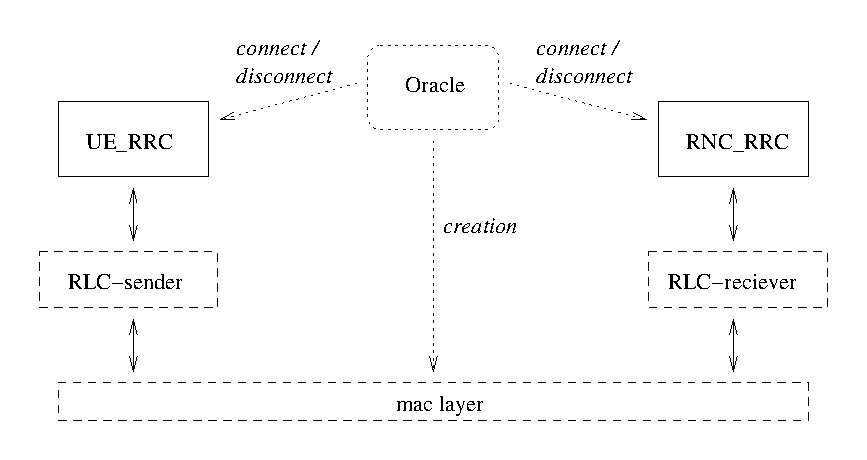
\includegraphics[height=4.5cm]{arch.eps}\\
  \caption{Structure of the specification}
  \label{arch}
\end{center}
\end{figure}

Each separate protocol entity is modeled as a EASN-process. The behavior
of RLC sender and RLC receiver processes are sketched in extended state
automaton form in the Figure \ref{rlcent1} and \ref{rlcent2}. 
In both the processes, a reception
of the disconnecting message from the above layer causes an immediate
termination, that is left out from the automata descriptions. In the
figures, transitions are specified in guarded command fashion, e.g.,
$from_rc?CR \Rightarrow ab:=1$ means that when receiving a $CR$ message from
user, the value of $ab$ is set to 1. MAC layer is specified with two
separate unreliable FIFO-buffers, one from sending RLC entity to
receiving entity and one for the other direction.

Full specification in both EASN and Promela format can be located at
\href{http://www.cs.helsinki.fi/u/mluukkai/easn/}{\tt
http://www.cs.helsinki.fi/u/mluukkai/easn/}.

%\begin{figure}
%\centerline{\psfig{figure=srlc.eps,height=6.0cm}}
%\caption{RLC sender}
%\label{rlcent1}
%\end{figure}

\begin{figure}
\begin{center}
  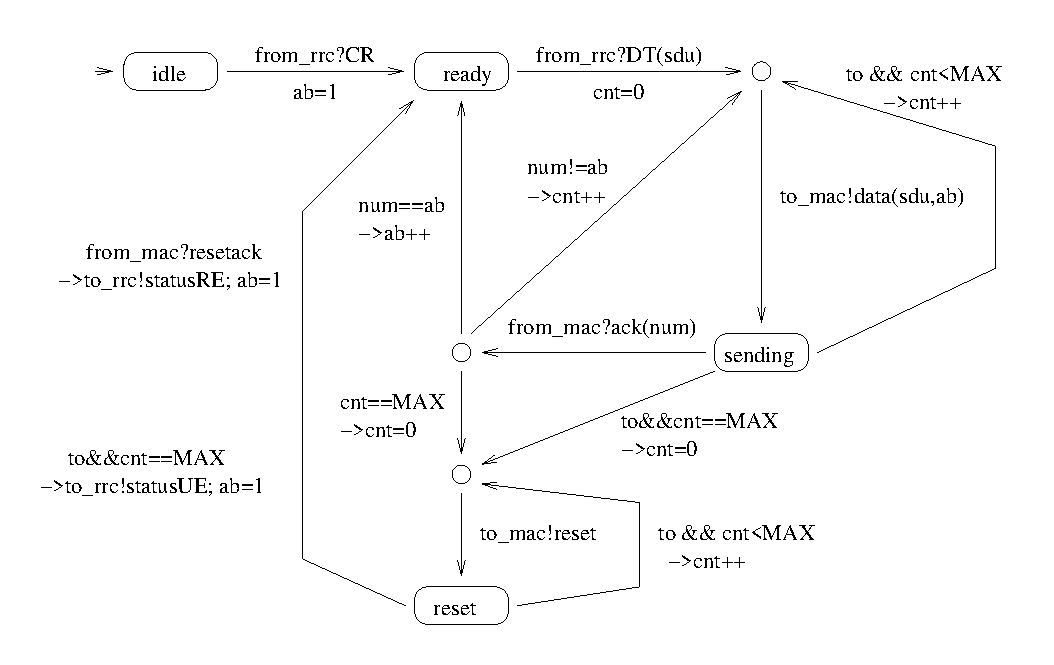
\includegraphics[height=6.0cm]{srlc.eps}\\
  \caption{RLC sender}
  \label{rlcent1}
\end{center}
\end{figure}


%\begin{figure}
%\centerline{\psfig{figure=rrlc.new.eps,height=5.5cm}}
%\caption{RLC receiver}
%\label{rlcent2}
%\end{figure}

\begin{figure}
\begin{center}
  \includegraphics[height=5.5cm]{rrlc.new.eps}\\
  \caption{RLC receiver}
  \label{rlcent2}
\end{center}
\end{figure}

One specific interesting point in the modeling has been the usage of
dynamic process creation and passing channel identifiers of the
dynamically created processes; these two features are supported by
both Spin and EASN. In this aspect this model differs from the
previous two reported in \cite{DSVV2000}, \cite{ICACSD} that used
labeled transition system specifications and a static structure where
the same RLC and MAC components are reused for the subsequent
connections.  The model of the RLC-protocol here follows the one
defined in the standard closely, since in reality different
MAC-connections do not share logical channels.

The actual way of modeling the dynamic aspects is the following:
\begin{enumerate}
\item At the start, three processes are created: the oracle, sending
      user and the receiving user.
\item Before starting a RLC-connection, the oracle creates a MAC-entity.
\item The MAC entity defines four local communication channels, two for both
        of the peer RLCs, and passes the channel identifiers to the oracle.
\item The oracle then passes the channel identifiers to the RRC entities which
       then start a RLC-connection setup.
\item Both the RRC entities then create RLC-entities, passing the
      corresponding MAC-channel identifiers to the created processes.
\item At the time of disconnection, both the RLC-entities and
       the MAC entity terminate. During the termination, the channels
        between MAC and RLCs  also vanish, since those were locally
        defined in the process that modeled MAC.
\item For the next RLC-connection, oracle starts all over again.
\end{enumerate}

The above modeling is possible due to the capability of the Promela or
EASN modeling languages to dynamically
create processes and pass channel identifiers between the processes.
From the verification point of view, it is also important that the terminated
protocol instances do not have any effect on the current state components of
the systems. That is actually the case if termination happens as in our model, 
where it is ensured that old entities have terminated
before new ones are generated.
 
\paragraph{Properties to be Proved and Verification Technique}
have any effect on the behavior of the protocol, a deadlock possibility
should exist after sending a list of $n$ SDUs, each consisting of just
a number 0. So, if we are able to show that the protocol does not deadlock
for any possible list of sent SDUs containing zeros, the protocol is free
of deadlocks in a general case where SDUs of any content are sent.

{\bf Detection of message duplication~~}
Let us assume that it is possible that protocol duplicates the $i$:th
SDU when sending a list $s_1,s_2,\ldots, s_n$ of SDUs. So, the
receiving user would be given SDUs $s_1,\ldots, s_i, s_i, \ldots s_n$.
The contents of the SDUs do not have any effect on the behavior of the
protocol. Thus in case of sending the list of SDUs $0^{i-1} 1 0^{n-i}$
(first 0 repeatedly $i-1$ times, then 1 and finally $n-i$ times 1),
the SDU consisting of the value 1 would be delivered to the receiving
user twice.  So, if we are able to show that the protocol delivers
exactly one SDU having content of 1 for any possible list of SDUs sent
of the form $0^i10^j$, the protocol in general does not duplicate SDUs
when SDUs of any content are being sent.

{\bf In-sequence delivery of messages~~}
Let us assume that it is possible that the protocol could change the
order in which $i$:th and $i+1$:th SDUs are delivered when sending a
list $s_1,s_2,\ldots, s_n$ of SDUs. So, the receiving user would be
given SDUs $s_1,\ldots, s_{i+1}, s_i, \ldots s_n$.  Since the contents
of the SDUs do not have any effect on the behavior of the protocol, in
case of sending the list of SDUs $0^{i}1^{n-i}$, the first SDU
consisting of 1 would be delivered before the last one consisting of
$0$.  So, if we are able to show that the protocol delivers all the
SDUs consisting of 0 before any consisting of 1 for all possible lists
of sent SDUs of the form $0^i1^j$, the SDUs are received in the same
order in which they were sent for a general case where SDUs of any
content are being sent.

The verification itself was conducted by modeling the RRC sender
entity in such a way that it sends the required type of SDUs, and in
the RRC receiver we then checked that the received SDU stream is of
right type.  As an example, a fraction of the RRC sender for the
in-sequence delivery verification is shown in the Figure
\ref{rrcsender}. So, first it sends SDUs with 0 as content and then,
nondeterministically at some point of time, it begins sending SDUs
with 1 as content. In this way, the reachability graph will contain
executions where every list of SDUs of the type $0^i1^j$ is
considered.

%\begin{figure}
%\centerline{\psfig{figure=rrcs.eps,height=1.5cm}}
%\caption{RRC sender entity for verification of in-sequence delivery }
%\label{rrcsender}
%\end{figure}

\begin{figure}
\begin{center}
  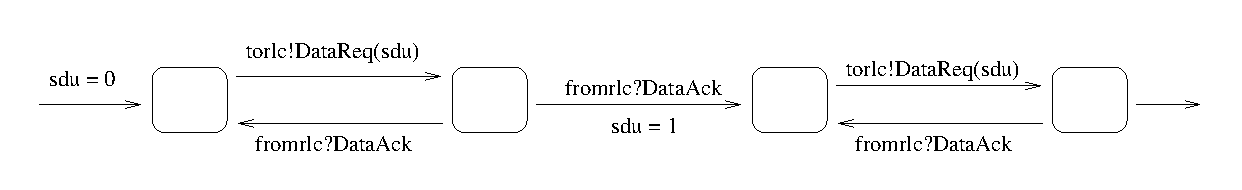
\includegraphics[height=1.5cm]{rrcs.eps}\\
  \caption{RRC sender entity for verification of in-sequence delivery}
  \label{rrcsender}
\end{center}
\end{figure}

\paragraph{Results of Verification}

We verified successfully all the properties of interest with several
different values for the maximum number of retransmissions. The tables
below summarizes some of the performance measures of the verification
both for EASN and for Spin when verifying an equivalent model of RLC
protocol.  The measurements listed are depth of the DFS-search, size
of the state vector (in bytes), number of states and transitions,
usage of memory (in Mega-Bytes), and time. The results are reported
separately for the various verification options which are (see
\cite{Spin} for a more specific description for the various options):

\begin{itemize}
\item $Noreduce$, meaning that the default optimizations in the
size of the stored state vector are turned off, 
\item $Bitstate$, Holzmann's bit-state hashing method
for approximating the set of reached states, and
\item $Collapse$, Wolper's hash compact method 
for approximating the set of reached states.
\end{itemize}

\begin{table}[ht]
%\caption{(easn/spin -a -DDEADLOCK -DMAXR=5 -DMAXD=5 ../../Test/rlc;)}
\caption{The deadlock detection}
\begin{center}
\begin{tabular}{||l|r|r|r|r|r|r|l|r||}
\hline
Options & depth & State & States & States  & Transi & Total & Time   & Tool\\
        &       & Vec   & Stored & Matched &  tions & Mem.  & (real)   &     \\
        &       & size  &        &         &        & (MB)  & (m:s)  &       \\
\hline
NoReduce & 3307 & 52& 116042& 193407& 309449& 8.515& 0:6.666 &Easn\\ %\cline{2-10}
 & 3307& 152& 116042& 193407& 309449& 10.870& 0:2.065&  Spin\\ \hline
 & 1646& 52& 54928& 38812& 93740& 5.215& 0:2.115& Easn\\ %\cline{2-10}
 & 1646& 152& 54928& 38812& 93740& 6.239& 0:0.663&  Spin\\ \hline
NoReduce & 3307& 0& 115601& 192508& 308109& 1.129& 0:4.383& Easn\\ %\cline{2-10}
 BitState & 3311& 152& 115747& 192800& 308547& 1.129& 0:1.420&  Spin\\ \hline
 BitState & 1638& 0& 54805& 38703& 93508& 1.813& 0:1.446& Easn\\ %\cline{2-10}
 & 1538& 152& 54709& 38555& 93264& 1.813& 0:0.476&  Spin\\ \hline
 Collapse & 1646& 28& 54928& 38812& 93740& 4.703& 1:54.781 &Easn\\ %\cline{2-10}
& 1684& 152& 55195& 38876& 94071& 5.318& 0:0.920& Spin\\ \hline
 NoReduce & 3307& 28& 116042& 193407& 309449& 7.695& 7:34.387& Easn\\ %\cline{2-10}
 Collapse & 3345& 152& 116327& 193517& 309844& 9.129& 0:2.917& Spin\\
\hline
\end{tabular}
\end{center}
\end{table}

\begin{table}[ht]
%\caption{(easn/spin -a -DDUPLICATE ../../Test/rlc;)}
\caption{Detection of message duplication}
\begin{center}
\begin{tabular}{||l|r|r|r|r|r|r|l|r||}
\hline
Options & depth & State & States & States  & Transi & Total & Time   &Tool\\
        &       & Vec   & Stored & Matched &  tions & Mem.  & (real) &    \\
        &       & size  &        &         &        & (MB)  & (m:s)  &      \\
\hline
NoReduce & 1231& 52& 301314& 649312& 950626& 19.677& 0:16.673& Easn\\ %\cline{2-10}
& 1231& 156& 301314& 649312& 950626& 26.742& 0:5.849&Spin\\ \hline
 & 673& 52& 61164& 36835& 97999& 5.522& 0:2.225& Easn\\ %\cline{2-10}
& 673& 156& 61164& 36835& 97999& 6.956& 0:0.736&Spin\\ \hline
 NoReduce & 1231& 0& 299023& 644079& 943102& 1.129& 0:10.693& Easn\\ %\cline{2-10}
BitState& 1231& 156& 298021& 642265& 940286& 1.129& 0:3.777&Spin\\ \hline
 BitState & 673& 0& 61136& 36828& 97964& 1.813& 0:1.517& Easn\\ %\cline{2-10}
 & 673& 156& 61002& 36731& 97733& 1.813& 0:0.492&  Spin\\ \hline
 Collapse & 673& 28& 61164& 36835& 97999& 4.908& 2:7.880& Easn\\ %\cline{2-10}
 & 673& 156& 62380& 37016& 99396& 5.830& 0:0.956& Spin\\ \hline
 NoReduce & 1231& 28& 301314& 649312& 950626& 17.424& 61:2.117&Easn\\ %\cline{2-10}
 Collapse & 1231& 156& 302530& 649493& 952023& 22.441& 0:8.552 & Spin\\
\hline
\end{tabular}
\end{center}
\end{table}

\begin{table}[ht]
%\caption{(easn/spin -a -DSEQUENCE ../../Test/rlc;)}
\caption{In-sequence delivery of messages}
\begin{center}
\begin{tabular}{||l|r|r|r|r|r|r|l|r||}
\hline
Options & depth & State & States & States  & Transi & Total & Time   &Tool\\
        &       & Vec   & Stored & Matched &  tions & Mem.  & (real) &    \\
        &       & size  &        &         &        & (MB)  & (m:s)  &    \\
\hline
 NoReduce & 1232& 52& 242596& 529114& 771710& 16.092& 0:13.773& Easn\\ %\cline{2-10}
& 1232& 156& 242596& 529114& 771710& 21.929& 0:4.648&Spin\\ \hline
 & 674& 52& 48022& 28983& 77005& 4.703& 0:1.741& Easn\\ %\cline{2-10}
& 674& 156& 48022& 28983& 77005& 5.830& 0:0.536&Spin\\ \hline
 NoReduce & 1258& 0& 241163& 525797& 766960& 1.129& 0:8.868& Easn\\ %\cline{2-10}
BitState & 1232& 156& 236052& 515455& 751507& 1.129& 0:2.985&Spin\\ \hline
 BitState & 674& 0& 48005& 28975& 76980& 1.813& 0:1.208& Easn\\ %\cline{2-10}
 & 674& 156& 47969& 28955& 76924& 1.813& 0:0.395&  Spin\\ \hline
 Collapse & 674& 28& 48022& 28983& 77005& 4.294& 1:19.238&Easn\\ %\cline{2-10}
 & 674& 156& 48918& 29117& 78035& 4.908& 0:0.759& Spin\\ \hline
 NoReduce & 1232& 28& 242596& 529114& 771710& 14.352& 36:56.357&Easn\\ %\cline{2-10}
 Collapse & 1232& 156& 243492& 529248& 772740& 18.345& 0:6.868 & Spin\\
\hline
\end{tabular}
\end{center}
\end{table}

As can be seen from the tables, EASN uses at most the same amount
memory that Spin uses, but as the sizes of the verification models
grow, EASN performs increasingly better than Spin, on memory-usage. We
have noticed upward of 20\% better memory performance from EASN, over
Spin. The price it has to pay is the increased run-times.

In crafting EASN from Spin, certain portions of the Spin source that
have to do with encoding of \emph{state} and its management have been
completely re-written for EASN, thereby making it possible to see
improvements in its memory performance. This approach was consciously
chosen, rather than simply translate ASN.1 types to appropriate
Promela-types. The fact that this new code-component in EASN has not
evolved as well, or for as long as the code from Spin that it replaces
into EASN, shows (rather clearly) in its run-times.

EASN employs Integer-Arithmetic for its computation of the hash-value
corresponding to its representation of the reached-state of the
system, through the use of the GNU Multi-Precision Arithmetic Package.
Spin, on the other hand, employs Polynomial-Arithmetic for the same
purpose. While Polynomial arithmetic can be faster than
multi-precision integer arithmetic, the latter allows EASN to compute
hash-values \emph{incrementally}. In the accompanying tables, notice
that EASN reports a state-vector size of 0 bytes, for the
\emph{BitState} runs as against non-zero values reported by Spin. For
these runs, Spin firstly represents the reached-state of the system in
a contiguous byte-array, and then computes two integer indexes based
upon that, into a bit-array, and sets the bits at the two indexes per
reached state. EASN, through its use of incremental computation for
the two indexes (from those corresponding to the state that the system
was in prior to evolving into its current state), does not require to
represent the reached-state explicitly. Refer \cite{easnspin} for a
complete discussion of the various design decisions, and their
rationale, as well as the related implementation aspects of EASN.

Even though this RLC case-study is not a large one, we have observed
that EASN simplifies the formal specification of large
telecommunication protocols or systems, since it involves one (manual
translation) step less (as against when using Spin), of having to
model the ASN.1 data through the use of Promela types.

\paragraph{``N-version'' Programming: SPIN and EASN systems}
Since the code base of EASN is derived from Spin system with changes
in the state vector representation and handling (an important and
critical part of the model checker), any discrepancy in the number of
states, etc. in the two systems can be explored to determine the
underlying causes. Such an effort has revealed the following anomalies
in the Spin system when working with the RLC model presented here.
\begin{itemize}
\item When using rendezvous channels, the compression mask was
  not completely restored on backward moves during the search.
  The correctness of the search was not affected, but the
  number of reached states became larger than necessary. This has been
  fixed in Spin 3.4.6 (29 March 2001).

\item In the {\tt s-hash} function, the computed hash value would
incorrectly also examine up to 3 extraneous bytes of the state vector
argument. This sometimes led to the re-exploring of some states.
\end{itemize}

\section{Conclusions}

In this article verification of the UMTS Radio link control protocol
\cite{3g-RLC} has been considered. This protocol implements several modes of
operation. For the verification, we selected the {\em reliable data
transfer service in the acknowledged mode}. The protocol was modeled
and verified using Spin, and EASN \cite{easnspin}, our Spin
\cite{Spin} based model checker for telecommunication systems. In
EASN, the data aspects of the protocol are modeled with ASN.1
\cite{asn1} while the control structures are the same as that of
Promela (Spin's input language). In order to compare EASN's
performance with that of Spin, we ran the verification in both the
systems. The data obtained from verification indicated that with
increase in the running time, EASN can manage with less memory than
Spin. The more complex data-types, and data-structures of EASN
contribute to its increased run-times.

We have already reported verification of some aspects of the RLC
protocol in \cite{DSVV2000} where we verified the simplified version
of the protocol, one where the disconnection phase was not
considered. In the earlier work we used labeled transition system
based modeling of the protocol. Within that framework, dynamic
creation of processes used here is not easy, so despite our earlier
model lacks the disconnection phase, it is slightly more complex than
the one we developed here. Furthermore, the dynamic aspect of the
modeling describes the 'reality' more closely, so we believe it to be
an extremely useful feature of both Spin and EASN systems.

\bibliographystyle{plain}
\bibliography{kirjalli}

\end{document}
% LocalWords:  UMTS EASN Luukkainen mattiEmail Vivek Shanbhag vivekEmail CSA
% LocalWords:  Microsystems Divyasree Gopinath gopiEmail ASN RLC Promela SDL
% LocalWords:  analysed livelocks LTL validator chan WCDMA OSI GPP SDU PDU RRC
% LocalWords:  PDUs SDUs NoReduce Easn BitState
